%%%%%%%%%%%%%%%%%%%%%%%%%%%%%%%%%%%%%%%%%%%%%%%%%%%%%%%%%%%%%%%%%%%%%%%%%%%%%%%%
%2345678901234567890123456789012345678901234567890123456789012345678901234567890
%        1         2         3         4         5         6         7         8

%\documentclass[letterpaper, 10 pt, conference]{ieeeconf}  % Comment this line out if you need a4paper

%\documentclass[a4paper, 10pt, conference]{ieeeconf}      % Use this line for a4 paper

\documentclass[letterpaper,10pt,conference,twocolumn]{ieeeconf} 
\IEEEoverridecommandlockouts
%\documentclass[11pt,reqno]{amsart} 
%\documentclass[conference]{IEEEtran}
%\documentclass[11pt,onecolumn]{IEEEtran}  

\usepackage{verbatim}
\usepackage[pdftex]{graphicx}
\usepackage{epsfig,subfigure}
\usepackage{amsmath,amssymb,amsfonts,bm,amscd} 
\usepackage{mathrsfs}
\usepackage{setspace}
\usepackage{fancyhdr}
%\usepackage{algorithm} 
\usepackage{psfrag}
\usepackage{cite}
\usepackage{tikz}
\usepackage[utf8]{inputenc}
\usepackage[ruled,vlined,linesnumbered,noresetcount]{algorithm2e}
\usepackage{pgfplots} 
\usepackage{pgfgantt}
\usepackage{pdflscape}
\usepackage[short]{optidef}
\pgfplotsset{compat=newest} 
\pgfplotsset{plot coordinates/math parser=false}

\newlength\fwidth

\newtheorem{theorem}{Theorem}[section]
\newtheorem{corollary}[theorem]{Corollary}
\newtheorem{lemma}[theorem]{Lemma}
\newtheorem{proposition}[theorem]{Proposition}
\newtheorem{conjecture}[theorem]{Conjecture}
%\theoremstyle{definition}
\newtheorem{definition}{Definition}[section]
\newtheorem{example}{Example}[section]
\newtheorem{assumption}{Assumption}[section]
%\theoremstyle{remark}
\newtheorem{remark}{Remark}[section]
\newtheorem{problem}{Problem}[section]
%\newtheorem{algorithm}{Algorithm}[section]

\newcommand{\scale}{0.8}
\newcommand{\norm}[1]{\left\Vert#1\right\Vert}
\newcommand{\abs}[1]{\left\vert#1\right\vert}
\newcommand{\set}[1]{\left\{#1\right\}}
\newcommand{\Real}{\mathbb R}
\newcommand{\Complex}{\mathbb C}
\newcommand{\eps}{\varepsilon}

% Mireille's defs
\newcommand{\Zero}{{\mathbf{0}}}
\newcommand{\CC}{{\mathbb C}}
\newcommand{\NN}{{\mathbb N}}
\newcommand{\RR}{{\mathbb R}}
\newcommand{\TT}{{\mathbb T}}
\newcommand{\UU}{{\mathbb U}}
\newcommand{\ZZ}{{\mathbb Z}}

\newcommand{\cA}{{\mathcal A}}
\newcommand{\cB}{{\mathcal B}}
\newcommand{\cC}{{\mathcal C}}
\newcommand{\cD}{{\mathcal D}}
\newcommand{\cE}{{\mathcal E}}
\newcommand{\cF}{{\mathcal F}}
\newcommand{\cG}{{\mathcal O}_{\mathcal P}}
\newcommand{\cH}{{\mathcal H}}
\newcommand{\cI}{{\mathcal I}}
\newcommand{\cK}{{\mathcal K}}
\newcommand{\cM}{{\mathcal M}}
\newcommand{\cN}{{\mathcal N}}
\newcommand{\cO}{{\mathcal O}}
\newcommand{\cP}{{\mathcal P}}
\newcommand{\cQ}{{\mathcal Q}}
\newcommand{\cS}{{\mathcal S}}
\newcommand{\cT}{{\mathcal T}}
\newcommand{\cU}{{\mathcal U}}
\newcommand{\cW}{{\mathcal W}}
\newcommand{\cX}{{\mathcal X}}
\newcommand{\cY}{{\mathcal Y}}

\newcommand{\rI}{{\mathrm{I}}}
\newcommand{\iI}{{\mathit{I}}}
\newcommand{\fI}{{\mathfrak{I}}}
\newcommand{\sI}{{\mathscr{I}}}
\newcommand{\sfI}{{\mathsf{I}}}
\newcommand{\eI}{{\EuScript{I}}}
\newcommand{\Bs}{{\mathscr{B}}}
\newcommand{\Ms}{{\mathscr{M}}}
\newcommand{\Us}{{\mathscr{U}}}
\newcommand{\Zs}{{\mathscr{Z}}}

\newcommand{\ks}{\kappa^{\star}}
\newcommand{\ms}{m^{\star}}
\newcommand{\vs}{v^{\star}}
\newcommand{\xs}{x^{\star}}
\newcommand{\ys}{y^{\star}}


\newcommand{\Tau}{\mathrm{T}}
\newcommand{\la}{\langle}
\newcommand{\ra}{\rangle}
\newcommand{\ol}{\overline}
\newcommand{\One}{\rm 1}
\newcommand{\p}{\partial}
\newcommand{\df}{\stackrel{\vartriangle}{=}}
\renewcommand{\Im}{\textup{Im }}
\newcommand{\Ker}{\textup{Ker }}
\newcommand{\conv}{\textup{co}}
\newcommand{\aff}{\textup{aff}}
\newcommand{\lin}{\textup{lin }}
\newcommand{\cone}{\textup{cone}}
\newcommand{\spn}{\textup{span}}
\newcommand{\rank}{\textup{rank}}
\newcommand{\inter}{\textup{int }}
\newcommand{\ri}{\textup{ri }}
\newcommand{\To}{\longrightarrow}
\newcommand\xqed[1]{%
  \leavevmode\unskip\penalty9999 \hbox{}\nobreak\hfill
  \quad\hbox{#1}}
\newcommand\demo{\xqed{$\triangleleft$}}


\title{\LARGE \bf
Trajectory Generation for Multiagent Point-to-Point Transitions via Distributed Model Predictive Control
}

\author{Carlos E. Luis% <-this % stops a space
% \thanks{*This work was not supported by any organization}% <-this % stops a space
\thanks{The author is with the Dynamic Systems Lab at the University of Toronto Institute for Aerospace Studies (UTIAS), Canada. Email: carlos.luis@robotics.utias.utoronto.ca}%
% \thanks{$^{2}$Bernard D. Researcheris with the Department of %Electrical Engineering, Wright State University,
%        Dayton, OH 45435, USA
%        {\tt\small b.d.researcher@ieee.org}}%
}

% Color definitions
\usepackage{xcolor,colortbl}
\definecolor{grey1}{RGB}{192,192,192}
\definecolor{grey2}{RGB}{178,178,178}
\definecolor{grey3}{RGB}{150,150,150}
\definecolor{grey4}{RGB}{119,119,119}
\definecolor{grey5}{RGB}{77,77,77}
\definecolor{green}{RGB}{112,173,71}
\definecolor{blue}{RGB}{68,115,196}
\definecolor{red}{RGB}{192,0,0}
\definecolor{yellow}{RGB}{255,192,0}

% Shortcuts
% \newcommand{\todo}{\textsf{\textbf{Todo (self-note): }}}
\newcommand{\question}{\textsf{\textbf{Question: }}}
\newcommand{\note}{\textsf{\textbf{Note: }}}

% Comment
\usepackage[colorinlistoftodos]{todonotes}

% Bold math
\usepackage{bm}

\begin{document}
\maketitle
\thispagestyle{empty}
\pagestyle{empty}


%%%%%%%%%%%%%%%%%%%%%%%%%%%%%%%%%%%%%%%%%%%%%%%%%%%%%%%%%%%%%%%%%%%%%%%%%%%%%%%%
\begin{abstract}
Here goes the abstract
\end{abstract}


%%%%%%%%%%%%%%%%%%%%%%%%%%%%%%%%%%%%%%%%%%%%%%%%%%%%%%%%%%%%%%%%%%%%%%%%%%%%%%%%


\setcounter{section}{0}
\section{Introduction}
\label{sec:introduction}
Generating collision-free trajectories when dealing with multiagent systems is a safety-critical task. In missions that require cooperation of multiple agents, such as surveillance \cite{vallejo2009multi}, crop inspection \cite{carbone2018swarm} and warehouse management \cite{guizzo2008three}, it is often desirable to safely drive the agents from their current locations to a set of final positions. Solving this problem, known as multiagent point-to-point transitions, is therefore an integral objective of any robust multiagent system.

There are two main variations of the multiagent point-to-point transition problem: the labelled or the unlabelled agent problems. In the former, each agent has a fixed final position that cannot be exchanged with other agents \cite{schouwenaars2001mixed, augugliaro2012generation}; in the latter, the algorithm is free to assign the goals to the agents, as to ease the complexity of the trajectories \cite{turpin2012decentralized}. This paper will focus on the labelled agent version. 

A common approach is to formulate an optimization problem. One of the first techniques developed relied on Mixed Integer Linear Programming (MILP), modelling collision constraints as binary variables \cite{schouwenaars2001mixed}. These methods, although viable, are computationally heavy and not suited for large teams.

More recently, Sequential Convex Programming (SCP) \cite{boyd2008sequential} has been used for faster computation compared to MILP. In \cite{augugliaro2012generation}, SCP is used to compute optimal-fuel trajectories of quadrotor teams. A decoupled version of that algorithm (dec-iSCP) is proposed in \cite{chen2015decoupled}, which has shorter computation time at the cost of suboptimal solutions. However, dec-iSCP is a sequentially greedy approach that makes the optimization problem harder to solve as more vehicles are added.

Discrete approaches divide the space in a grid and use known discrete seach algorithms \cite{preiss}. Other mixed approaches combine optimization techniques and predefined behaviours to manage collisions \cite{tang2018complete}. Lyapunov barrier functions have also been used to compute multiagent collision-free trajectories \cite{wang2017safety}.

Distributed optimization approaches can effectively include pair-wise distance nonlinear constraints \cite{bhattacharya2011distributed}. Furthermore, the distributed nature reduces the computational effort with respect to centralized approaches. A new solution to the problem is proposed in this paper, based on distributed model predictive control (DMPC) \cite{camponogara2002distributed}. Synchronous implementation of DMPC \cite{dai2017distributed,wang2014synthesis}, allows the agents to solve their optimization problems in parallel. Previous work on DMPC shows its capabilities in multiagent tasks, such as formation control \cite{van2017distributed,sayyaadi2017decentralized}, but not explicitly for point-to-point transitions as highlighted in Fig.~(\ref{fig:30_random}).

The rest of the paper is organized as follows: Section II formulates the optimization problem solved by each agent, and Section III formalizes the DMPC algorithm for multiagent point-to-point transitions. Finally, Section IV presents simulation results of DMPC and compares its performance with dec-iSCP.

\begin{figure}[t]
	\centering
	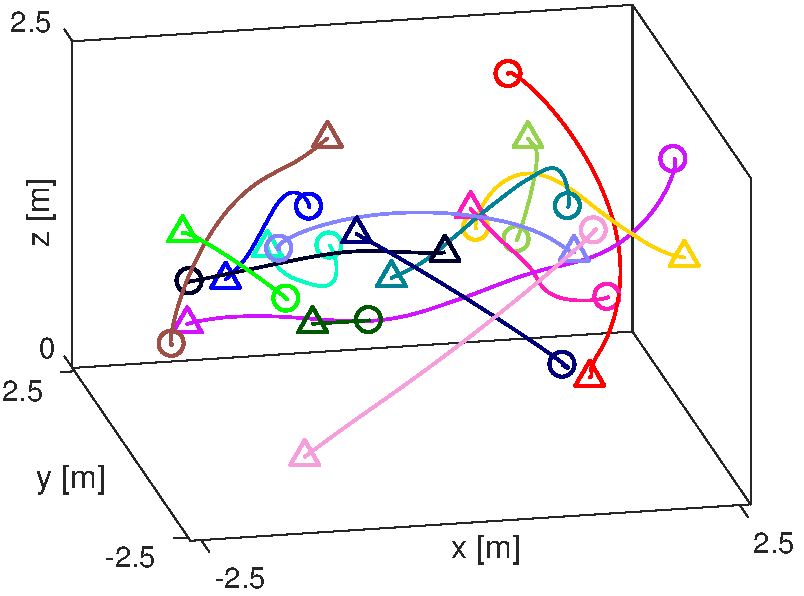
\includegraphics[width=0.45\textwidth]{figures/30_rand}
	\caption{A 15-vehicle point-to-point transition solved using our DMPC algorithm. The initial and final positions (denoted with triangles and circles, respectively) were chosen randomly within a convex volume of $5 \times 5 \times 2$m. The agents were required to maintain a minimum distance of 0.75m of each other throughout the trajectory. Even in this highly cluttered dynamic environment, the proposed algorithm is capable of quickly finding a collision-free trajectory for all agents.}
	\label{fig:30_random}
\end{figure}







\section{Problem Statement}
\label{sec:formulation}

This section introduces the different components of the optimization problem to be solved. The formulation must accomplish the following criteria:
\begin{enumerate}
	\item Drive all agents from their starting positions to their desired final positions.
	\item Respect a minimum pair-wise distance throughout the trajectory (collision constraint).
	\item The position and acceleration of the agents must be within specified boundaries.
\end{enumerate}

\subsection{The model}
Each agent is modeled as a unit mass in $\RR^3$. The formulation is identical for each agent, so the $i$ subscript to distinguish agents' states is omitted. For simplicity, we use an abbreviated matrix representation as if the vectors were one-dimensional. 
\begin{equation}
\label{eqn: model}
\begin{bmatrix}
p[k+1]\\
v[k+1]
\end{bmatrix} = \begin{bmatrix}
1 & h\\
0 & 1
\end{bmatrix} \begin{bmatrix}
p[k] \\
v[k]
\end{bmatrix} + \begin{bmatrix}
h^2/2 \\
h
\end{bmatrix}a[k]
\end{equation}
Vectors $p$, $v$ and $a$ are the discretized position, velocity and acceleration of the mass at time step $k = {0,1,\ldots,K-1}$, with $K$ being the length of the horizon and $h$ the time step duration in seconds. A compact representation is given by
\begin{equation}
x[k+1] = Ax[k] + Bu[k] 
\end{equation}
where $x \in \RR^{6}$, $A \in \RR^{6\times 6} $, $B \in \RR^{6\times 3}$ and $u[k] \in \RR^{3}$. Expanding the model derives in
\begin{equation}
\label{eqn:expand}
\begin{aligned}
x[1] &= Ax[0] + Bu[0]\\
x[2] &= A^2x[0] + ABu[0] + Bu[1]\\
&\vdots\\
x[K] &= A^{K}x[0] + A^{K-1}Bu[0] + \ldots + Bu[K-1]
\end{aligned}
\end{equation}
From Eqn.~(\ref{eqn:expand}), we can write the position sequence $P \in \RR^{3K}$ as an affine function of the input sequence $U \in \RR^{3K}$,
\begin{equation}
\label{eqn:model}
P = A_0X_0 + \Lambda U
\end{equation}
where $X_0 \in \RR^{6K}$ is the repeated sequence of initial states, and $\Lambda \in \RR^{3K \times 3K}$ is defined as
\begin{equation}
\Lambda = \begin{bmatrix}
\Psi B & 0 & \ldots & 0\\
\Psi AB & \Psi B & \ldots & 0 \\
\vdots & \ddots & \ddots & \vdots \\
\Psi A^{K-1}B & \Psi A^{K-2}B & \dots & \Psi B 
\end{bmatrix}
\end{equation}
with matrix $\Psi = \begin{bmatrix}
I_3 & 0
\end{bmatrix}$ selecting the first three rows of the matrix products (those corresponding the position states). 
Lastly, $A_0 \in \RR^{3K \times 6}$ is the propagation of the initial states
\begin{equation}
A_0 = \begin{bmatrix}
\Psi A & \Psi A^2 & \ldots & \Psi A^K
\end{bmatrix}^\top
\end{equation}

\subsection{Objective function}
The objective function has three main components: trajectory error, control effort and input variation. A similar formulation can be found in \cite{ru2017nonlinear}.

\subsubsection{Trajectory error penalty}
this term drives the agents to their goals. We want to minimize the error between the position at the final time step of the prediction horizon $p[K]$, and the desired final position $p_d$. The error term is 
\begin{equation}
e = \norm {p[K]-p_d}_2
\end{equation}
which can be casted into a quadratic cost function of the input sequence, using Eqn.~(\ref{eqn:model})
\begin{equation}
\label{eqn:error}
J_e = U^\top(\Lambda^{\top} \tilde{Q} \Lambda)U - 2(P_d^\top \tilde{Q} \Lambda -  A_0X_0 \tilde{Q} \Lambda)U
\end{equation}
Matrix $\tilde{Q} \in \RR^{3K \times 3K} $ is a positive semidefinite matrix that weights the error at each time step. Given that we want to enforce the trajectory to \textit{end} at the desired reference, then
\begin{equation}
\tilde{Q} = \begin{bmatrix}
0 & \ldots & 0 \\
\vdots & \ddots & \vdots \\
0 & \ldots & Q
\end{bmatrix}
\end{equation}
where $Q \in \RR^{3 \times 3}$ is chosen as a diagonal positive semidefinite matrix that weights each coordinate of the position vector at the last time step of the horizon.

\subsubsection{Control effort penalty}
we also want to minimize the total control effort throughout the trajectory, using the quadratic cost function
\begin{equation}
\label{eqn:input}
J_u = U^\top \tilde{R} U 
\end{equation}
Similarly, $\tilde{R} \in \RR^{3K \times 3K} $ is positive semidefinite and weights the penalty on control effort,
\begin{equation}
\tilde{R} = \begin{bmatrix}
R & 0& \ldots & 0 \\
0 & R & \ldots & 0 \\
\vdots & \ddots & \ddots & \vdots \\
0 & 0 & \ldots & R
\end{bmatrix}
\end{equation}
with $R \in \RR^{3 \times 3}$, a diagonal positive semidefinite matrix.

\subsubsection{Input variation penalty}
this term is used to minimize variations of the acceleration, leading to smooth trajectories in position. Define the quadratic cost
\begin{equation}
\label{eqn:delta}
J_\delta = \sum_{k=0}^{K-1}\norm{u[k]-u[k-1]}^2
\end{equation}
To transform Eqn.~(\ref{eqn:delta}) into a quadratic form, define $\Delta \in \RR^{3K \times 3K}$
\begin{equation}
\Delta = \begin{bmatrix}
I_3 & 0 & 0 & \ldots & 0 & 0 \\
-I_3 & I_3 & 0 & \dots & 0 & 0 \\
0 & -I_3 & I_3 & \ldots & 0 & 0 \\
\vdots & \ddots & \ddots & \ddots & \vdots & \vdots\\
0& 0 & 0 & \ldots & -I_3 & I_3
\end{bmatrix}
\end{equation}
and define a vector $U_{-1} \in \RR^{3K}$ to include the term $u[-1]$ (input applied in the previous time step of the trajectory)

 \begin{figure*}
 	\centering
 	
 	\begin{subfloat}{
 		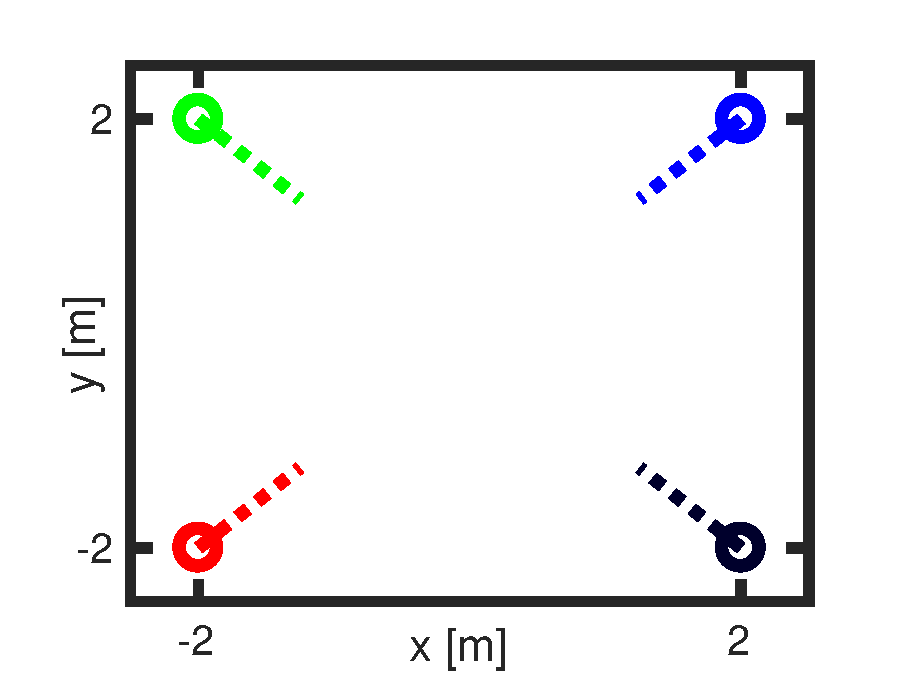
\includegraphics[width=0.26\textwidth]{figures/rail_a}}
 	\end{subfloat} \hspace{-5ex}
 	%
 	\begin{subfloat}{
 			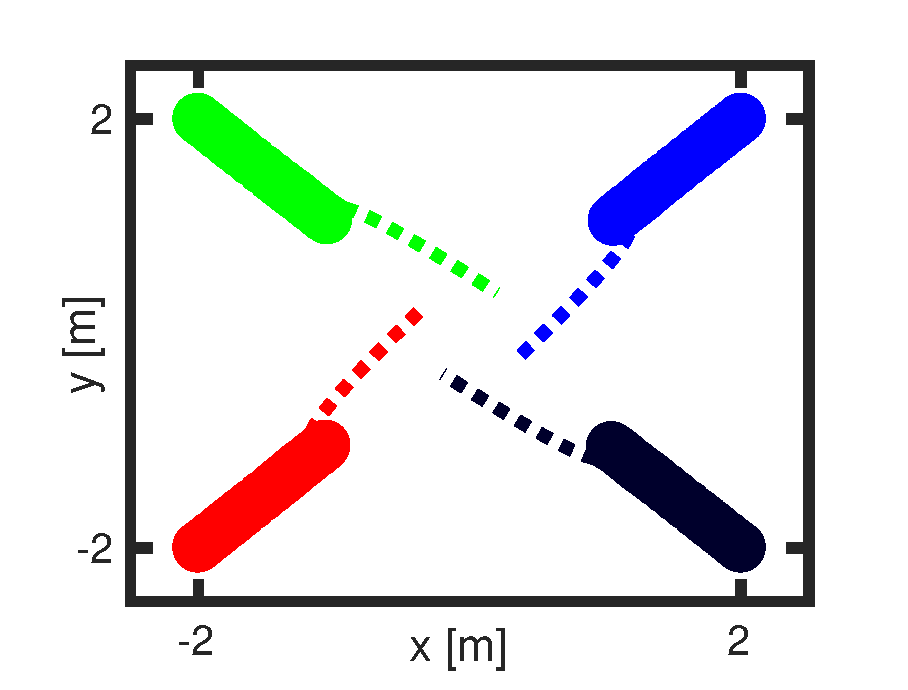
\includegraphics[width=0.26\textwidth]{figures/rail_b}}
 	\end{subfloat} \hspace{-5ex}
 	%
 	\begin{subfloat}{
 			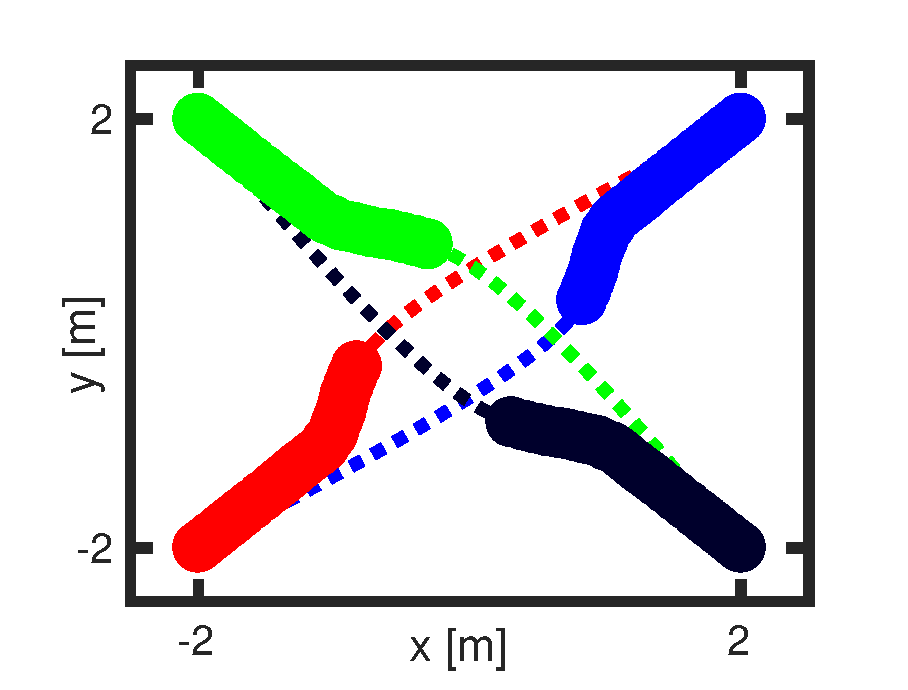
\includegraphics[width=0.26\textwidth]{figures/rail_c}}
 	\end{subfloat} \hspace{-5ex}
 	%
 	\begin{subfloat}{
 			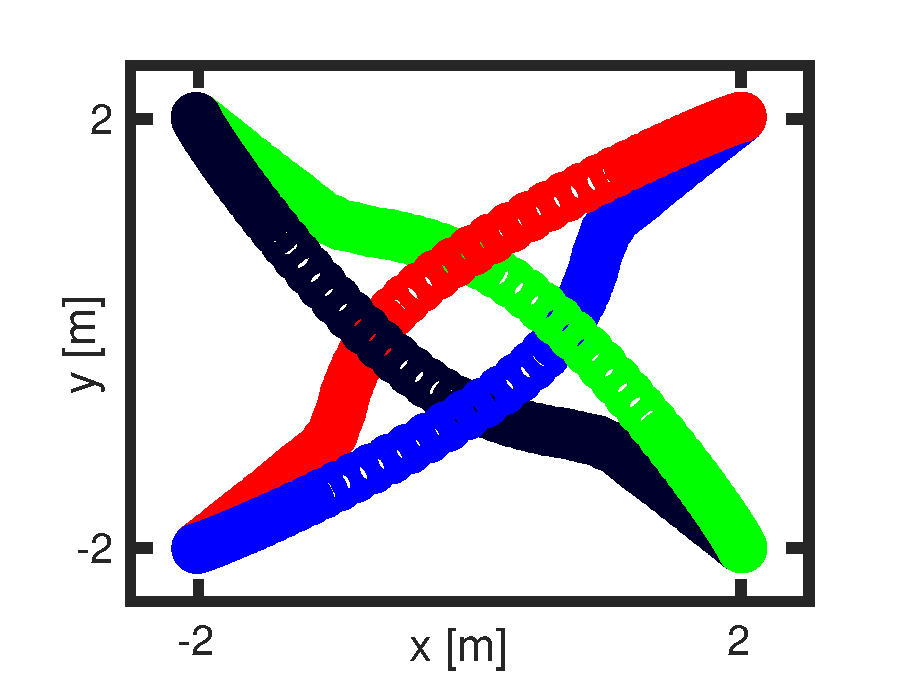
\includegraphics[width=0.26\textwidth]{figures/rail_d}}
 	\end{subfloat} 
 	\caption{4-vehicle position exchange scenario in 2D, solved using DMPC. The vehicles predict future collisions and slow down to safely circumvent the congested area. The result is a successful point-to-point transition, respecting all the constraints of the problem. }
 	\label{fig:four}
 \end{figure*}
\begin{equation}
U_{-1} = \begin{bmatrix}
u[-1] & 0 & \ldots & 0
\end{bmatrix}^\top
\end{equation}
Finally, we write Eqn.~(\ref{eqn:delta}) in quadratic form as
\begin{equation}
\label{eqn:var}
J_\delta = U^\top (\Delta^\top \tilde{S} \Delta) U - 2(U_{-1}^\top \tilde{S} \Delta )U
\end{equation}	
where $\tilde{S} \in \RR^{3K \times 3K}$ is positive semidefinite of the form

\begin{equation}
\tilde{S} = \begin{bmatrix}
S & 0& \ldots & 0 \\
0 & S & \ldots & 0 \\
\vdots & \ddots & \ddots & \vdots \\
0 & 0 & \ldots & S
\end{bmatrix}
\end{equation}
with $S \in \RR^{3 \times 3}$, a diagonal positive semidefinite matrix.

The total cost function $\mathcal{J}$ is obtained by adding together Eqns.~(\ref{eqn:error},\ref{eqn:input},\ref{eqn:var})
\begin{equation}
\begin{aligned}
\mathcal{J}(U) &=  U^\top (\Lambda^{\top} \tilde{Q} \Lambda + \tilde{R} + \Delta^\top \tilde{S} \Delta) U \\
 & -2 (P_d^\top \tilde{Q} \Lambda -  A_0X_0 \tilde{Q} \Lambda + U_{-1}^\top \tilde{S} \Delta)U
\end{aligned}
\end{equation}	

\subsection{Collision avoidance}
To procure collision avoidance, each agent uses information of the most up-to-date prediction horizon of every other agent ($p_j$). Adding constraints on all the time steps with expected collisions was found to be overly restrictive, reducing the probability of finding a feasible solution. Hence, agent $i$ enforces collision constraints with all neighbours only on the \textit{first} time step $k$ with predicted collisions,
\begin{equation}
\label{eqn:coll}
\norm{p_i[k]-p_j[k]}_2 \geq r_{min} \quad \forall j = 1,2,\ldots,N \quad i \neq j
\end{equation}	
The quadratic constraint in Eqn.~(\ref{eqn:coll}) is linearized using a Taylor series expansion about the previous iterate $q$ of the predicted position horizon of agent $i$ ($p_i^q$),
\begin{equation}
\label{eqn: taylor}
\norm{p^q_i[k] - p_j[k]}_2 + \frac{(p_i^q[k]-p_j[k])^\top}{\norm{p^q_i[k] - p_j[k]}_2}(p_i[k]-p_i^q[k]) \geq r_{min}
\end{equation}
The only variable in Eqn.~(\ref{eqn: taylor}) is $p_i[k]$, then it can can be expressed as
\begin{equation}
\label{eqn: bla}
(p_i^q[k]-p_j[k])^\top p_i[k] \geq \rho_j
\end{equation}
with
\begin{equation}
\begin{aligned}
\rho_j &= r_{min}\norm{p^q_i[k] - p_j[k]}_2 - \norm{p^q_i[k] - p_j[k]}_2^2 \\
& \hspace{1em}+ (p_i^q[k]-p_j[k])^\top p^q_i[k]
\end{aligned}
\end{equation}
Now, cast Eqn.~(\ref{eqn: bla}) into an affine function of the input $U$,
\begin{equation}
\Upsilon_j \Lambda U_i \geq \rho_j - \Upsilon_j A_0 x_i[0]
\end{equation}
where $\Upsilon_j \in \RR^{1 \times 3K}$ is defined as
\begin{equation}
\Upsilon_j = \begin{bmatrix}
0_{1\times 3k} & (p_i^q[k]-p_j[k])^\top & 0_{1 \times 3(K-1-k)}
\end{bmatrix}
\end{equation}
Finally, introduce $A_{coll,j} \in \RR^{1 \times 3K}$ and $b_{coll,j} \in \RR$
\begin{equation}
\label{eqn: coll}
A_{coll,j} = \Upsilon_j \Lambda ; \quad b_{coll,j} = \rho_j - \Upsilon_j A_0 x_i[0]
\end{equation}
The complete collision constraint for agent $i$, $A_{coll} \in \RR^{(N-1) \times 3K}$ and $b_{coll} \in \RR^{(N-1)}$, can be obtained by stacking vertically the matrices in Eqn.~(\ref{eqn: coll}) for all the $N-1$ neighbours of agent $i$.


\subsection{Physical Limits}
The agents must remain within a specified volume and respecting acceleration limits, hence inequality constraints must be enforced both in the position and acceleration at each time step of the prediction horizon. Let $p_{min}, p_{max}, a_{min}, a_{max} \in \RR^3$ be the physical limits of the system. Define $P_{min}, P_{max}, U_{min}, U_{max} \in \RR^{3K}$
\begin{equation}
\begin{aligned}
P_{min} = [p_{min} \ldots p_{min}]^\top; \quad  P_{max} = [p_{max} \ldots p_{max}]^\top \\
U_{min} = [a_{min} \ldots a_{min}]^\top; \quad  U_{max} = [a_{max} \ldots a_{max}]^\top
\end{aligned}
\end{equation}
Then, the physical limits constraints are formulated as
\begin{equation}
\begin{aligned}
P_{min} &\leq \Lambda U \leq P_{max} \\
U_{min} &\leq  U \leq U_{max}
\end{aligned}
\end{equation}

\subsection{Convex optimization problem}
The complete inequality constraints for agent $i$ are obtained by stacking vertically the collision avoidance and physical limits constraints. At each time step of the trajectory, agent $i$ solves the following convex optimization problem to update its prediction horizon
\begin{mini}|l|
	{U}{\mathcal{J}(U)}{}{}
	{\label{eqn:convex}}{}
	\addConstraint{A_{in}U}{\leq b_{in}}
\end{mini}
If collisions are predicted, the problem would have $6K+N-1$ inequality constraints, otherwise the number is reduced to $6K$. The formulation in Eqn.~(\ref{eqn:convex}) results in a Quadratic Programming problem that can be computed efficiently. 
	
	
\section{Distributed Model Predictive Control Algorithm}
\label{sec:problemStatement}
The proposed DMPC algorithm for point-to-point transitions is outlined in Alg. 1. It requires as input several parameters used in Section~\ref{sec:formulation}: $h$, $K$, $N$, $Q$, $R$, $S$, $p_{min}$, $p_{max}$, $a_{min}$, $a_{max}$, $r_{min}$. Also, a simulation duration $T$, in seconds, needs to be specified. In line 1, the algorithm initializes a list of prediction horizons for all vehicles by specifying linear trajectories from initial positions to final positions. While it hasn't converged or the maximum number of iterations is not exceeded, the algorithm goes through each time step of the trajectory ($k_T = {1,...,K_T}$ with $K_T = T/h + 1$), and through every agent, solving the corresponding QP as derived in Eqn.~(\ref{eqn:convex}). If a solution is found, then it executes a state propagation by applying the first input of the optimization variable $U$, to the model in  Eqn.~(\ref{eqn: model}) (lines 6-8). If a solution was not found due to infeasibility of the problem (or exceeding the maximum number of iterations of the QP solver), then a heuristic approach was introduced to retry solving the problem.

\begin{algorithm}
	\SetKwData{Left}{left}\SetKwData{This}{this}\SetKwData{Up}{up}
	\SetKwFunction{Union}{Union}\SetKwFunction{FindCompress}{FindCompress}
	\SetKwInOut{Input}{Input}\SetKwInOut{Output}{Output}
	\Input {Initial and final positions, DMPC parameters}
	\Output {Position, velocity and acceleration trajectories for all vehicles}
	
	$l \leftarrow$ Initialize predictions
	
	\While{trials $<$ max and not converged}{
		\ForEach{trajectory time step $k_T = {1,...,K_T-1}$}{
			\ForEach{agent $i = {1,...,N}$}{
				$a_i[k_T] \leftarrow$ Solve QP - Eqn.~(\ref{eqn:convex})
				
				\eIf{QP solved}{
					$p_i[k_T],v_i[k_T] \leftarrow$ Propagate States
					
					$l \leftarrow$ Update Prediction Horizon
				}{
				exit loop}	
		}
		\If{QP not solved}{
			$Q \leftarrow$ Increase $Q$
			
			$trials \leftarrow$ $trials +1$ 
			
			exit loop
		}
	}
	
	\uIf{QP solved and all vehicles reached goal}{
		converged $\leftarrow$ true;
	}
	\uElseIf{QP solved and not all vehicles reached goal}{
		$Q \leftarrow$ Increase $Q$
		
		$trials \leftarrow$ $trials +1$ 
	}			
}
\eIf{converged}{
	$[p,v,a] \leftarrow$ Interpolate for higher resolution
	
}
{$[p,v,a] \leftarrow \emptyset$ 
}
\KwRet {[p,v,a]}
\caption{DMPC for Point-to-Point Transitions}
\end{algorithm}

\subsection{Heuristic approach for improved feasibility}
The heuristic approach considers two different scenarios for choosing the values of the $Q$ matrix.
\begin{enumerate}
	\item No collisions are detected in the horizon: the agent has a more aggressive behaviour towards the goal. Uses matrix $Q_{agg}$ with high enough value to procure good trajectory tracking.
	\item Collisions in the horizon: a more conservative behaviour is required to safely circumvent future collisions. Use matrix $Q_{coll}$ with reduced diagonal values with respect to $Q_{agg}$.
\end{enumerate}

Although this approach helps in some cases, in others the conservativeness of the agents is counterproductive to avoid collisions. In those cases, (lines 11-14) a more aggressive behaviour during predicted collisions is enforced, and the algorithm tries to solve the problem with the new matrix $Q_{coll}$. In some other cases, the conservative behaviour can avoid collisions but is unable to reach the waypoint within the simulation duration $T$, in those cases a more aggressive behaviour is also induced to the agents and the problem is resolved (lines 17-19). 

Convergence of Alg. 1 is declared when the trajectories for all agents respect all the constraints, and the point-to-point transition was completed within $T$ seconds. If the algorithm coverged, the last step (lines 20-21) is to interpolate the resulting trajectory to obtain a better resolution (say, time step $T_s = 0.01s$).
\section{Main Results}
\label{sec:results}

\section{Conclusions}
\label{sec:conclusions}


\bibliographystyle{IEEEtran}
\bibliography{IEEEabrv,reference}

% \clearpage
% \color{grey1}{
% \section{INTRODUCTION (0.5)}
%\label{sec:introduction}
\begin{itemize}
\item Introduce reference tracking/trajectory formation problem and applications, and point out the importance of achieving high performance in impromptu/unrehearsed/one-shot manner.
% \question Should we keep tracking as the targeting problem? yes.
\item Objective of this research: To formalize a neural-network-based control architecture that is generalizable to different platforms. This includes characterizing conditions which the architecture is applicable, guidelines for efficient feature selection, as well as conditions that allows for improving efficiency of training
\item Challenges in standard controller design (link to difficulties in tunning, modeling unknown factors, capability of achieving good performance on arbitrary trajectories).
\begin{itemize}
\item Tunning PI and PID controller based on step response (\r{A}str\"{o}m and H\"{a}gglund, 2004): rules not universal, may need more accurate models in some cases, may be conservative in some cases
\item Point out cases where controller is not accessible (off-the-shelf products)
\end{itemize}
\item Introduce incorporation of machine learning (summarize/model experience and enable taking advantage of previous experience -- using knowledge not just from starting of a trial); introduce neural network and advantages (machine learning, robotics, control), and point out the potential of modeling non-linearities.
%\item In contrast with image classification and natural language recognition problems, dynamical systems are governed by relatively more well-defined functions (?), which can be exploited in DNN design especially feature selection process; based on theory to guide feature selection (also, comment from practical aspect -- convenient to test etc.).
%\item Brief introduction of neural-network based architectures in literature
%\item Angela -- add somewhere, something like: Finding the optimal structure of DNNS as been considered for other application areas such as image classification, speech, ...
\item Discuss efficient feature selection or extraction or optimization techniques (e.g., convolutional structure and PCA -- link to incorporation of invariance in input) developed in image classification. (In control literature, not much discussion in efficient feature selection; most focus is on control architecture design and training -- check this)
\item Brief introduction of summer research work, and refer to Related Work section for details (inverse-dynamics-based model approach, and achieved error reduction about 40\%-50\% on average) \cite{DNNimpromptuTrack}. \color{blue}{Fig. 1. Summer research paper architecture illustration}\color{grey1}
\item Contributions: (1) with respect to summer research work, justifications of design decisions and generalization of the approach; (2) with respect to intelligent control, an approach of efficiently selecting features for inverse-dynamics-modeling-based architectures; (3) with respect to general control, formulation of an enhancement-based architecture with guidelines can be potentially continently adapted to industrial applications \textbf{(?)}
\item Roadmap: (1) introduce recent work (summer research), (2) review of intelligent control literature (point out concerned points that are alleviated with current approach), (3) formulation/generalization of the approach proposed in summer research, (4) Illustration with simulation/experiment example
% \item Potential introduction points
% \begin{itemize}
% \item Connection with PID tunning: (\r{A}str\"{o}m and H\"{a}gglund, 2004) PID popular controller. Tunning methods based on step responses (to determine parameters). Proposed approach enhances of PID based control based on step responses (to select input feature -- $r$ and difference vs direct signal).
% \end{itemize}
\end{itemize}

\section{Background (1)}
%\label{sec:background}
\subsection{Related Work}
%\label{subsec:relatedWork}
\begin{itemize}
\item Summarize neural-network-based and neural-network-inverse-modeling-based architectures and training procedures in literature 

\todo Check what happened in recent 20 years. Abbeel and Goldberg.

%\question Is it necessary to discuss other neural-network-based architectures?
\begin{itemize}
\item Brief summary of architectures (point is to show stability advantages of current approach)
\item Architectures with inverse-modeling and discussion 
\item Training methods and discussion
\end{itemize}
\item Other recent work with experimental results

%\question Include details here or briefly summarize in introduction? here.
\begin{itemize}
\item Forward dynamics learning and LQR-based/MPC approaches (stability -- proposed approach, under special conditions (no feedback of reference and current state), can be modeled by feedfoward static network and is stable)
\end{itemize}
\end{itemize}
\subsection{Details of Previous Work}
\label{subsec:previousWork}
%\item Description of summer research work
\begin{itemize}
\item Proposed approach: control architecture and training process \color{blue}Fig. 2. Block diagrams illustrating control architecture and training\color{grey1}
\item Results: testing platform (quadrotor) and achievements (average of 40-50\% error reduction on 30 trajectories)
\item Note the features of the design here (3 things helps with stability, difference used to introduce translational invariance -- training efficiency, ...); separate the ones that are practical and the ones that are backed with theoretical results (refer to the result section)
\item Comparisons with other approaches:
\begin{itemize}
\item Less prone to stability issue for both training and testing phrases as compared with \textit{feedback error learning approach}
\item More goal-directed as compared with \textit{general inverse learning} approach, not necessary to compute Jacobian as compared with \textit{specialized learning approach}, does not depend on a well-tuned controller as compared with \textit{feedback error learning approach}
\end{itemize}
\item Limitations (motivations of this paper): feature selections are based on experimental tryouts, tested on one system and assumptions are not explicitly identified
\end{itemize}

%learning in general, neural nets based, inverse based, summer research paper

%a review of what is done and achieved in summer research paper

\section{PROBLEM STATEMENT (0.125)}
%\label{sec:problemStatement}
The problem to be addressed in this paper is to formulate the deep-neural-network-based approach developed in Ref(summer research paper) in a framework that is generalizable to other applications. This includes a platform-independent formulation for both feature selection and model training, identification of assumptions implicitly applied in the implementation, as well as characterizing conditions under which the efficiency of training process can be improved. 
%Summer research good results; decisions are experimentally obtained
%Formulate the approach such that it can be generalized to other applications/platforms; identify assumptions (stable inverse, difference-learning, unnecessity of using past reference (relative degree = degree, or use current internal state feedback) )

% \section{ASSUMPTIONS (0.25}
% \label{sec:assumptions}
% \begin{itemize}
% \item Invertability (?)
% \end{itemize}

\section{RESULTS (2-3)}
%\label{sec:results}
% \note I included discussions associated with the transfer function (will remove if not necessary). The reasons I thought this might be useful are that (1) it is an alternative for identifying input-output to neural networks that uses a series of states rather than the current internal state, and (2) it may help to discuss the point about learning difference. % Conclusion: do not include detailed derivations


% sunday: this part + validity, figure list, 
\begin{itemize}
% \item Define feedback loop dynamics in the form of controllable controllable canonical form (with initial conditions)
% \item Derive $z$-transform and discuss the effect of initial condition; arrive at the transfer function with assumption of zero initial values
\color{grey1} 
\item State normal form with the expression of $u$ dependency
\item Roadmap (point to generalization to nonlinear system discussion)
\end{itemize}




%Mathematical preliminaries (form of feedback loop system SISO)
% \noindent\question Explanation of choosing SISO for derivations?

% \noindent\question Is controllable canonical form sufficient for discussion (this would be easier to discuss the TF derivations, if it would be used for discussing learning difference)? Is it alright to assume strictly proper system ($r>$0)? Or, should it be kept as general ($\mathbf{A}$,$\mathbf{b}$,$\mathbf{c}$)?

% \noindent\question Assumption on invertability?

\subsection{Validity/Efficiency/Efficacy of approach}
%\label{subsec:stability}
\begin{itemize}
\color{grey1}
% \item Normal form of forward and inverse dynamics
% \item Discussion on stability (connection between state-space ($\textrm{eig}(Q)$) and transfer function (zeros) conclusions)
\item Comments the applicability of the approach requires (1) there is a well-defined relative degree and (2) stable inverse dynamics

\noindent\todo Find practical example of cases/platforms where relative degree is defined and not defined

\item For linear system, stability of zero dynamics can be checked by step input response tests (minimal-phase) 

\noindent\todo Check finiteness of relative degree for discrete linear system
\item For nonlinear systems, there are conditions which the constant input stability does not imply stability of general inputs

\noindent\todo Check reference cited in Chapter 3.3 of the textbook
\item For nonlinear systems, it is also possible to relative degree may be variable for different operational ranges

\noindent\todo Think about simulation for this point
\end{itemize}
%\vspace{1em}
% \fbox{
% \begin{minipage}{24em}
\textbf{Key message}
\begin{itemize}
\color{grey1}
\item The validity of the proposed approach requires a well-defined relative degree (inherent delay) and stable zero dynamics.
\item For nonlinear systems, the relative degree may be locally defined.
\end{itemize}
% \end{minipage}}


% ---------------------------------------------
\subsection{Feature selection}
%\label{subsec:featureSelection}
\begin{itemize}
\color{grey1}
\item Point out that the experimental tryouts involved in the summer research paper; the system is tuned for the quadrotor platform. The object here is to draw insights from the theoretical result that allows for both efficient feature selection and identification of assumptions that were implicitly made in the implementation.
\item Discussion on the feature selection based on state-space representation, which has following advantages
\begin{itemize}
\item Account for disturbances and initial errors
\item Allow for feedforward neural network structure. Benefits: From implementation perspective, feedforward NNs are easier to train; from control perspective, neural network is static, and thus BIBO stable.
\item Does not need to know order (based on knowledge about $r$, which can be determined experimentally)
\item Potential reduction of input dimension; ($n+1$ for state-space, $2n-r-1$ for transfer function)
\end{itemize}
\item Comment on the derivation depends on internal state; if not known, either use state estimation to construct full state or use an alternative expression derived based on transfer function
\item Introduce the expression based on transfer function (does not need internal states, but require potentially more states, less capable of disturbance rejection)
% \item Identify dependencies of current reference state (state-space and transfer function)
% \item Comment that if current internal state is accessible, the dimension of input features can be reduced
\item Conclusions of nonlinear systems (relative degree)
\item Practical comments:
\begin{itemize}
\item State-space: comment on identification of relative degree $r$
\item $z$-transform: if possible, outline experimental procedure for determining the degree $n$; otherwise, comment that this needs to be chosen conservatively (more states)
\item Note about the loop frequencies: Lower outer loop frequency needed for not causing instabilities. The identification of $r$ should be based on outer loop rate not the rate of data collection (at inner loop rate)
\end{itemize}
\end{itemize}

%with state-space, only need to know the relative degree

%otherwise, conservatively chose number of future states

%dependence on past input states
% \subsection{Applicability of using feedfoward neural networks}
% \begin{itemize}
% \item Benefits: From implementation perspective, feedforward NNs are easier to train; from control perspective, neural network is static, and thus BIBO stable 

% \todo Think about the case with feedback; make this point stronger
% \item The applicability of this structure depends on whether the inverse dynamics has dependency on past reference states; this is possible in two scenarios (1) having access to current internal state such that the state-space approach can be used, and (2) the order and relative order of the system are equal $r=n$.

% \question The second conclusion is based on the linear SISO system; I am not sure if it is good to state it here. Is it possible to assume nonlinear systems can have linearized feedback loop dynamics like the point-ahead-linearized unicycle system?
% \end{itemize}

%unnecessity of using past reference (relative degree = degree, or use current internal state feedback) 


% \fbox{\begin{minipage}{24em}
\textbf{Key messages}
\begin{itemize}
\color{grey1}
\item There are two approaches of identifying dependencies based on system inverse dynamics. One approach is based on state-space representation and leads to expression involving feedback of $\mathbf{x}(k)$, while a second approach is based on $z$-transform and leads to an expression involving series of $u$ and $y$.
% \begin{itemize}
% \item Number of inputs: former has less inputs, especially for cases with (large $n$ and) small $r$ 
\item Initial condition and disturbance rejection: if loop stable, effect of initial condition decays. Former additionally compensates for non-zero initial conditions and disturbances with feedback (better performance).
%\item Simplification of training process: latter possible to learn difference if zero steady state error for unity DC gain (point of next section)
% \end{itemize}
\end{itemize}
% \end{minipage}}


% -----------------------------------
\subsection{Learning difference}
%\label{subsec:learningDifference}
\begin{itemize}
\color{grey1}
\item Comment on being able to learn difference the possibility of having ``translational invariance'' in the model, which helps the efficiency of modeling and the training process
\item Comment following derivation aims to establish a practical connection between the conditions which this is possible and the properties of the control loop that can be easily tested/designed
\item State-space and $z$-transform based discussion of possibility of learning difference
\item Comment the condition is implied from achieving unity DC gain

\todo Theoretical insights of the connection + conclusion for the nonlinear case
% \question Should the results for state-space (the left-eigenvalue form) be included here? No, unless complete.
\end{itemize}

\textbf{Key message}
\begin{itemize}
\item The training dataset size can be potentially optimized by learning the input-output of the inverse dynamics relative to current state. This optimization is possible for cases where the feedback control loop has unity DC gain.
\end{itemize}
%further simplification of using yd to approximate current yc to enable offline learning

% \subsection{Possibility of offline computation}
% \label{subsec:offlineComputation}
% \begin{itemize}
% \item Current state can be approximated by current desired state for possibility of offline adjustments of reference trajectory
% \item Feasibility is discussed in the summer research paper

% \noindent\question I am not sure if this should be mentioned here since it is discussed in the summer research paper and verified with experiments
% \end{itemize}

% \subsection{Nonlinear systems}
% \label{subsec:learningDifference}
% \begin{itemize}
% \item Relative degree derivation
% \item Comment on connections with linear system derivations

% \todo More details
% \end{itemize}

\section{SIMULATION/EXPERIMENT (2-3)}
% show a case when the inverse (zero dynamics for linear case, or a nonlinear scenario) is not stable
%\label{sec:simulationExperiment}
% \noindent Figures...
\begin{itemize}
\item Point 1: Zero-dynamics stability
\begin{itemize}
\item Simulation: Linearized system with feedback loop transfer function $\frac{k_ps+k_d}{(1+k_d)s+k_p}$ with stable pole and unstable zero. \color{blue}{Fig. 2D trajectory plot ($y$ and $y_d$ versus time) showing instability}
\end{itemize}
\item Point 2: Disturbance and initial error compensation with feedback of $\mathbf{x}$
\begin{itemize}
\item Experimental comparison 1: (1) with feedback of current state and (2) using series of $y_d$ instead. \color{blue}{Fig. Error plots in two directions showing benefits of using current state feedback.}\color{grey1}
\item Note: try to avoid the case requiring recurrent structure (dependencies on previous $u$) (?)
\end{itemize}
\item Point 3: Learning difference condition and comparison
\begin{itemize}
\item Experimental comparison 2: (1) with steady state error and (2) without steady state error. \color{blue}{Fig. Error plots for case with constant input or arbitrary.}\color{grey1}
\item Experimental comparison 3: (1) with difference and (2) without difference. \color{blue}{Fig. Scatter plots of training points that correspond to similar performance}\color{grey1}, or \color{blue}{Fig. Error plots showing performance comparison for same number of training points.}
\end{itemize}
\end{itemize}


% \begin{itemize}
% \color{grey1}
% \item unstable zero dynamics (a simulation): linear (trajectory, error, etc. showing the learned function) and nonlinear (operational range change...think about generation of this case)
% \begin{itemize}
% \item Linear system 
% \end{itemize}
% \item disturbance: error plot(s) of using state feedback versus not
% \item learning difference: trajectory plots showing performance (figure/performance measure) or profile plots, operating range coverage scatter plots in some input space (difference in number of points needed) - a 1D/2D example here (smaller dim easier to illustrate)?
% \item ...
% \item \todo think about what are the cases can be generated with the platforms
% \end{itemize}

%\noindent\question Unicycle as the main problem instead of quadrotor; since the point is to show generalization, (also able to show unstable case by controller selection) (?)

\subsection{Simulation/Experiment setup}
\begin{itemize}
\color{grey1}
\item Introduce problem, plant model \color{blue}{Fig. Experimental setup illustration}\color{grey1}
\item Introduce study cases
\item Roadmap and summary table (case, controller, input-output of NN)
\end{itemize}

\subsection{Derivations}
\begin{itemize}
\color{grey1}
\item Derive feedback-loop dynamics
\item Inverse dynamics stability
\item Feature selection
\item Condition of learning differences
\end{itemize}

\subsection{Training details}
\begin{itemize}
\color{grey1}
\item Data generation
\item Structure of training
\end{itemize}

\subsection{Discussions}
\begin{itemize}
\color{grey1}
\item Zero-dynamics stability
\item Disturbance and initial error compensation
\item Condition for learning difference
\item Training efficiency with difference-learning
\end{itemize}

\section{CONCLUSIONS (0.25)}
\label{sec:conclusions}
\begin{itemize}
\color{grey1}
\item Formulation summary and identification of conditions for applicability (echo problem statement)
\item Summarize simulation results
\end{itemize}

\section*{REFERENCES (0.25-0.5)}

\color{grey5}
\section*{Reminders}
\begin{itemize}
% \item DNN
% \item Check Abstract word count
\item General guidelines for the training process [Result Section Intro]: ``Should this be mentioned here with the essential input features in Section  IV-B before you start the discussion on improving the efficiency of training in Section IV-C''
\item Robustness of assuming $y=y_d$
\item Rewrite the part about feedforward vs. recurrent networks
\item Title: the word `design'
\item unity DC gain of nonlinear systems
% \item update simulation figure
% \item make `dsl' plot smaller, update title of trajectory plots
\item learning difference figure need to re-run and include longer time
% \item define unseen trajectory
% \item revise the subsection on ss and tf comparison
% \item move figures to top of pages
\end{itemize}
% }
\end{document}
